\graphicspath{{chapters/02/images}}
\chapter{Introduction}

\section{Sleep}
Sleep is a naturally recurring, reversible physiological state of reduced consciusness, sensory perception, and voluntary motor activity characterized by altered brain wave patterns, diminished responsiveness to external stimuli and distinctive physiological and behavioral changes \cite{sleep}.
It is crucial for cognitive functioning, emotional well-being and overall health in humans and many other organisms.
There is an extensive overlap between sleep mechanisms and the neurophysiology of learning and memory processes, which provides a strong rationale for theories supporting a functional link between sleep and learning systems \cite{sleep-cognitive}.

  \subsection{Common features of sleep across organisms}
  Sleep can be considered as a vulnerable state that is incompatible with behaviors that nourish and propagate species.
  Because of this sleep must fulfill some universal vital function \cite{sleep-across-species}.
  It can be considered as a state that increases the efficiency of behavior by regulating its timing and by reducing energy use.
  It reduces activity and body and brain metabolism while allowing a high level of responsiveness to external stimuli with respect to hibernation or torpor.
  For example, the human brain can continuously process sensory signals and trigger complete awakening to significant stimuli within a few milliseconds.

  \subsection{Sleep in humans}
  In humans and other mammals, sleep is characterized by a reduction of voluntary motor activity and decreased responsiveness to external stimuli and is composed of two alternating phases: rapid eye movement (REM) sleep and non-REM (NREM) sleep \cite{cognitive-neuroscience-of-sleep}.
  REM sleep is characterized by Ponto-geniculo-occipital PGO waves, theta synchrony, increased acetylcholine, reduced levels of monoamines and increased transcription of plasticity-related genes, which together contribute to freely occurring bidirectional plasticity long-term potentiation LTP and depotentiation in the hippocampal complex.
  During NREM sleep this is extended to the neocortex, where orderly neuronal reactivation events in phase with slow wave delta activity facilitate the events that convert early LTP to long-lasting LTP.\\

    \subsubsection{REM sleep}
    REM sleep is necessary for strong, lasting improvements and its effects on memory consolidation are circuit-specific \cite{rem-review}.
    Synaptic gains are specific to circuits involved in a learning task and do not transfer to other processing fields.
    Moreover, spontaneous increases in REM sleep follow training and precede large increases in performance during learning.
    However, it is not the total REM sleep time that is fundamental for learning, but rather its relative augmentation after a task is performed that allows for better learning.\\
    A characteristic signature of REM sleep is PGO waves, which are generated in the pons and travel to the lateral geniculate nucleus and the occipital cortex.
    They increase in density during intensive learning, and their density is correlated with task retention.
    They are hypothesized to be a potent regulator of synaptic plasticity in the hippocampus and amygdala, and they are comprised of large, synchronous excitatory waves of glutamate that terminate directly on forebrain targets.\\
    The hippocampus is fundamental for the formation of new memories, in fact, memory consolidation is the transfer of hippocampal plasticity to long-term storage sites in the neocortex.
    Long-term potentiation is easily induced during sleep in this area, facilitating task retention.\\
    Active neurons during waking are reactivated during sleep with an increased firing rate with respect to ones that were not activated.
    These neurons have an increased co-activation during hippocampal large irregular activity LIA which occurs during NREM and a structured replay of the waking running sequences during REM sleep.
    This happens in a theta-specific pattern concordant with the induction of LTP and its reversal during the REM sleep state.
    Place cells in the hippocampus fire dependent on the electroencephalographic (EEG) theta rhythm during active waking.
    This suggests that LTP could be induced with physiologically feasible stimuli if timed to the naturally occurring theta activity.

    \subsubsection{NREM sleep}
    NREM sleep is characterized by a slow wave activity (SWA) in the electroencephalogram \cite{nrem-review}.
    Learning during waking amplifies slow waves which allow for a reactivation of neurons that were involved in learning or encoding during theta states on accelerated and condensed time scales.
    This increase in slow waves is associated with increased waking task requirements demanded from the same area neocortex.
    The function of these reactivations is memory consolidation: it strengthens memory circuits, facilitating LTP in the hippocampus and neocortex.\\
    The fact that slow wave-dependent processing affects synaptic weights is subject to further study, but the best evidence of this effect is a rise in the amplitude of slow waves after extended waking experience that becomes attenuated again after a period of slow wave activity ensues and the decline in evoked potentials across sleep.
    These results support the role of slow wave processing in reducing the strength of synapses.
    The work presented here will try to build a model to explain how this reduction in synaptic strength and slow wave activity can be used to explain changes in the activity patterns of neurons in the olfactory system of the honey bee during sleep.

  \subsection{The honey bee as a model for sleep}
  Insects are emerging as a model for sleep research: they have a simple nervous system, they are easy to manipulate, they have a short life cycle and they are equipped with a genetic toolbox \cite{sleep-mammals}.
  Sleep seems to be of fundamental importance also for insects: in the honey bee sleep deprivation at night impairs the precision of waggle dance signaling \cite{waggle-sleep-deprivation} and the probability of successfully returning to the hive the following day \cite{sleep-honeybee-consolidation}.
  In the honey bee no typical mammalian EEG signal is present, so the identification of sleep-like states in insects is based on behavioral criteria like inactivity and the presence of a specific body posture, an increased threshold to arousing stimulation and a rebound in the sleep-like state as a consequence of sleep deprivation.\\
  Bees are the organism of choice for this work because of their highly developed brain with a 10-fold increased number of neurons with respect to Drosophila.
  They can fulfill complex navigation and communication tasks.
  The effect of sleep on a memory task seems to focus on extinction learning.
  Extinction learning refers to the process of learning that a previously learned association is no longer valid.
  Sleep promoted in the bees the formation of extinction memories \cite{bee-extinction-memory}.
  Acquisition of a classical conditioned response is thought to occur at the level of the antennal lobe \cite{memory-acquisition-al}.
  Other networks like the mushroom bodies might specifically support extinction memory, but their role has still to be scrutinized.

    \subsubsection{Sleep in the honey bee}
    In the honey bee long-term, extracellular, single-unit recordings from optomotor intraneurons in the optic lobes show oscillations in their sensitivity to moving visual stimuli that display properties typical of a circadian rhythm \cite{neuronal-correlates-sleep-bee}
    In fact, the sensitivity of neurons to light of a given wave-lenght varies according to the time of day with a sigmoid response-log intensity function with positive slope shifts towards higher intensities in the evening.
    This fluctuation in sensitivity represents an endogenous circadian oscillation.
    The circadian changes in neuronal sensitivity are related to the sleep-wakefulness rhythm of the honey bee, showing increased sensitivity during the subjective day (when the animal's motor activity is high).\\
    Moreover, arousal stimuli restore the neurons' sensitivity, making the existence of a general arousal system plausible, with a mechanism similar to the one found in cats.
    During sleep the bee can let parts of their sensory systems become largely insensitive, provided that they can be reactivated quickly.\\
    Honey bees display a deep-sleep stage, where antennae become immobile.
    Repeated presentations of an odor for which the bees already learned a representation resulted in a better performance in retention tests \cite{bee-odor-retention}.\\
    After the deep-sleep state, spontaneous antennal activity can be observed, with a function that still needs to be explored \cite{bee-sleep-description}.
    However, it can be noted how the spontaneous activity of individual neurons in the visual system correlates with the time-courses of the antennal movement.

\section{The olfactory system of the bee}
As the antennal lobe is considered the site of memory acquisition, the focus of this work will be to build a model of this part of the olfactory system of the honey bee and explore the effects of sleep on it.\\
The olfactory system is a complex neuronal network organized in multiple highly interconnected neuropils organized hierarchically.
Each of these neuropils is a complex circuit comprising thousands of neurons with feedback and feed-forward interaction within and across them \cite{olfactory-coding-honeybee}.
The local interaction within neuropils and the global interaction between them results in the neural correlates of an olfactory stimulus.

  \subsection{Neuroanatomy}
  A schematic representation of the olfactory system of the honey bee is shown in figure \ref{fig:olfactory-system}.
  Four antennal nerve (AN) tracts (T1 to T4) compose the axon of the olfactory receptor neurons ORNs that innervate the first olfactory neuropil of the bee brain, the antennal lobe (AL).
  Each ORN innervates a single glomerulus.
  All ORNs expressing the same olfactory receptor converge to the same of the 160 glomeruli of the AL.
  After processing in the AL the information is relayed to higher-order processing centers via the medial and lateral antennal lobe tracts (m- and l-ALT), two antiparallel tracts projecting to the ipsilateral mushroom body and lateral horn.

  \begin{figure}
    \centering
    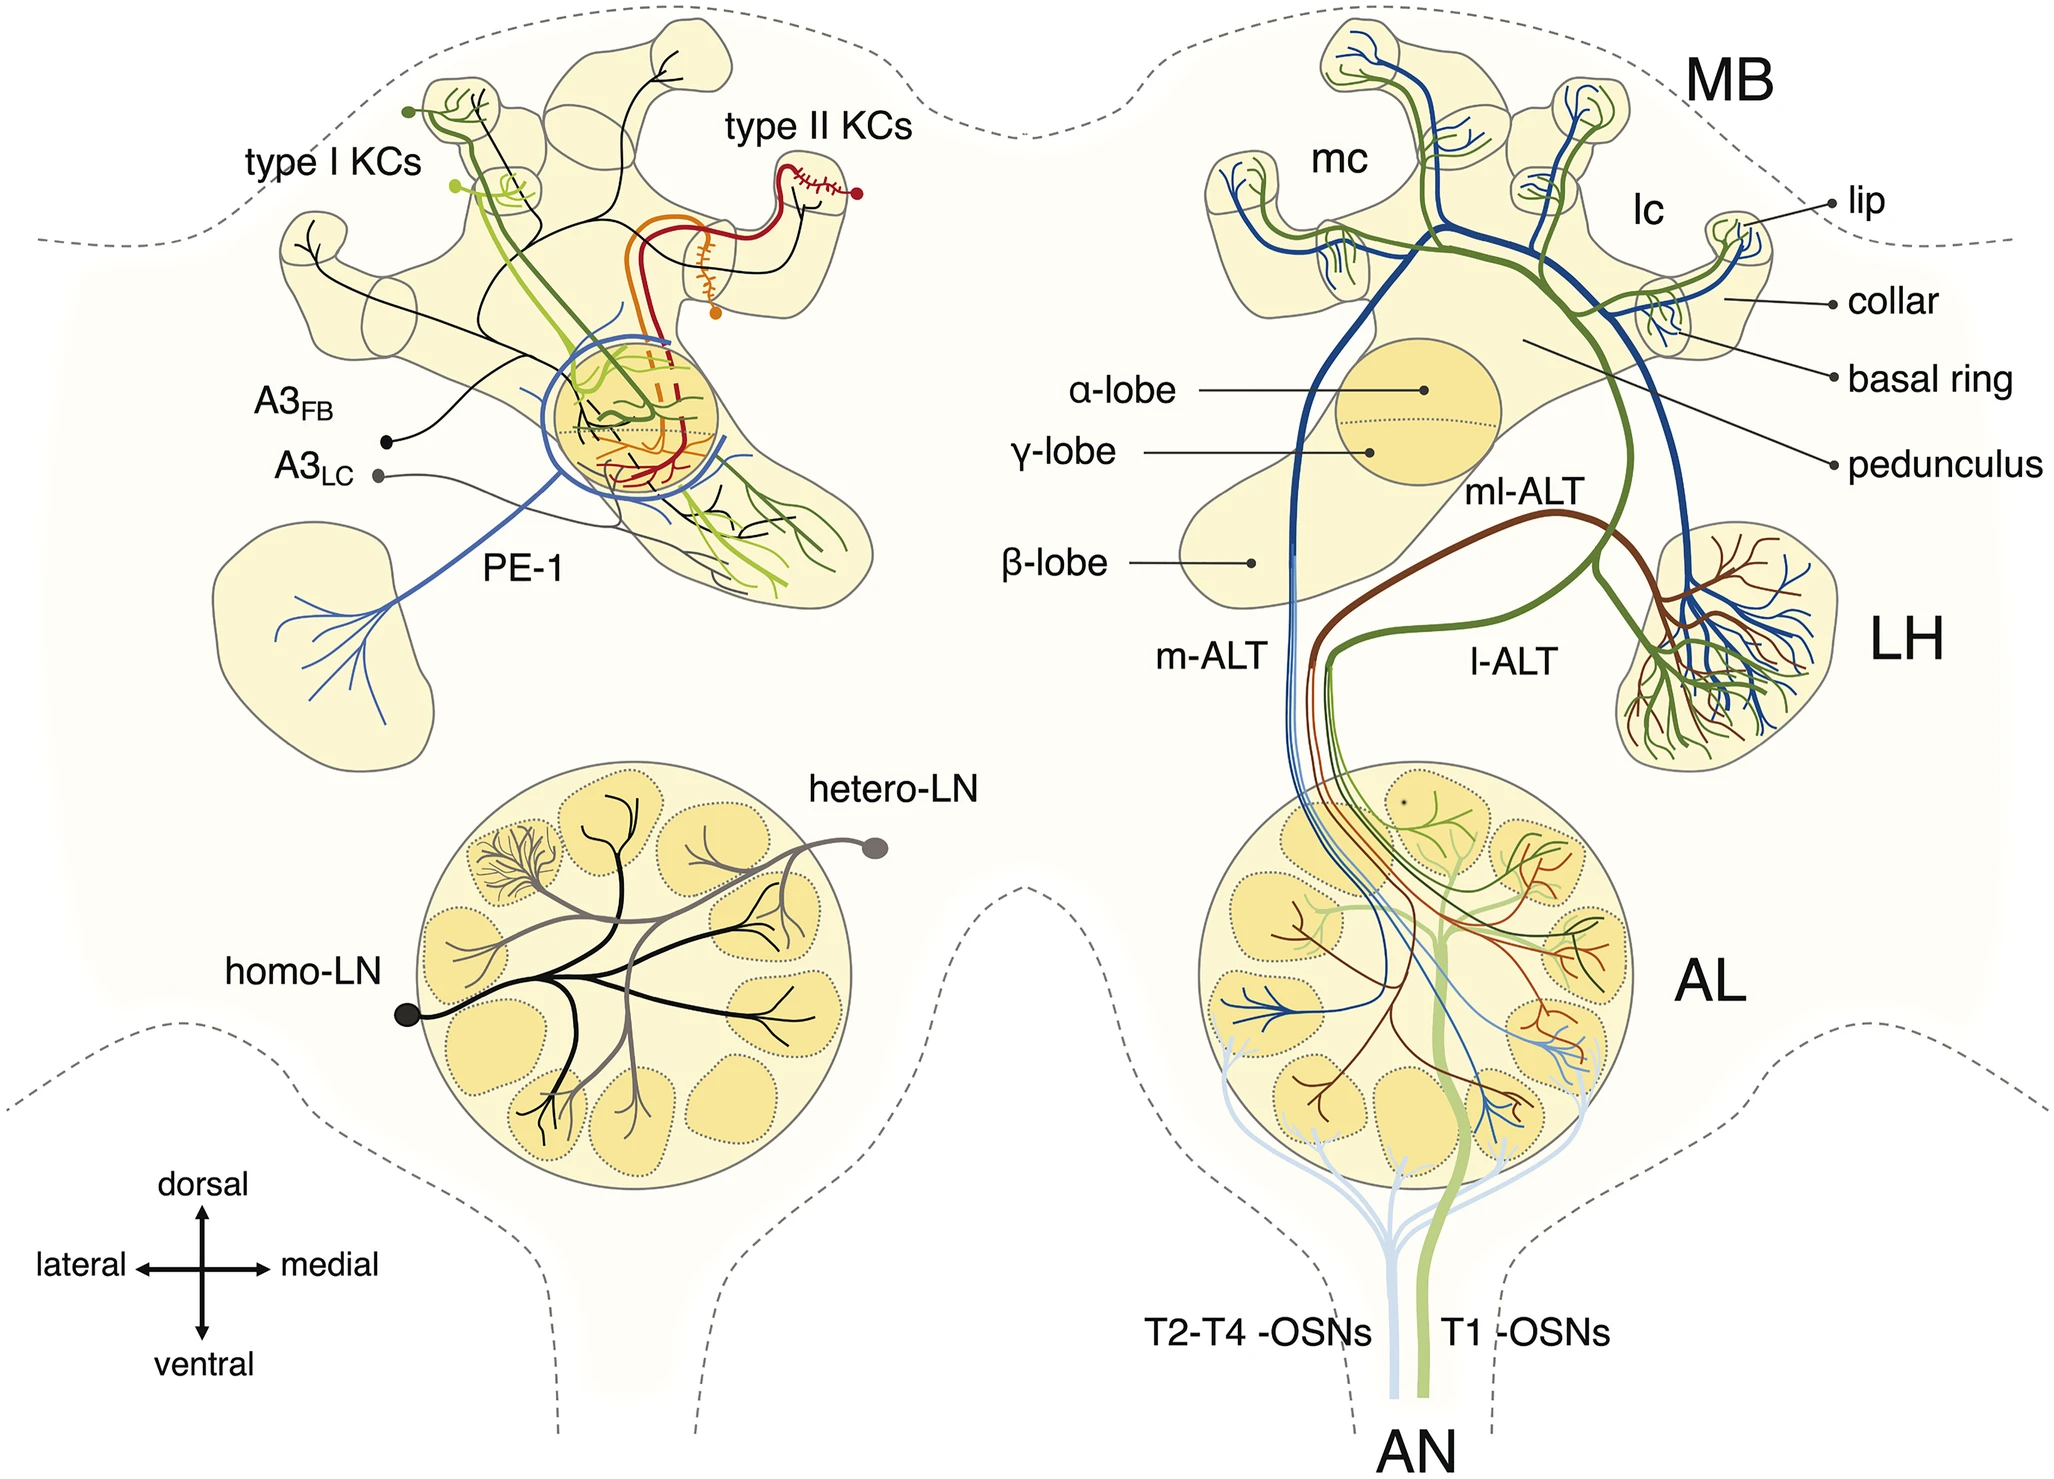
\includegraphics[width=0.8\textwidth]{organisation_olfactory_system}
    \caption{Schematic representation of the olfactory system of the honey bee, image taken from \cite{olfactory-coding-honeybee}.}
    \label{fig:olfactory-system}
  \end{figure}

  \subsection{Odor reception}
  The peripheral olfactory organs of the bee are the antennae, where the ORNs are located.
  Each antenna is composed of a scapus, a pedicel and a flagellum, the last of which hosts the sensilla, structures containing several olfactory receptor neurons.
  Volatile molecules reaching the honey bee antennae enter the sensillar pores and diffuse until they reach the ORNs' dendritic membrane.
  The sensillar lymph in this area contains olfactory binding proteins and odorant degrading enzymes.
  The former facilitates the transition of the odorant into a liquid environment and transports it toward the olfactory receptors, while the latter has a role in the degradation of odorants, promoting signal termination by limiting the time an odorant is present in the sensillar lymph and preventing olfactory receptors' saturation.\\
  The olfactory receptors ORs are located in the dendritic membrane of the ORNs and they are the main drivers for the molecular receptive response of the system.
  They are C-terminus-out seven-transmembrane-domain proteins containing a ligand-binding domain, which are active as heterodimers with the co-receptor.
  Their expression level varies during the honeybee development and they are influenced by experience.
  Olfactory coding initiates with the biochemical interaction between the ligand and the olfactory receptor, starting odor signal transduction.
  The specificity varies between receptors, allowing for a limited number of receptors to encode a great number of olfactory combinations.
  Moreover, the specific affinity of a receptor for a particular odorant allows for a concentration-dependent response so that minute variations in stimulus nature and concentration can produce significant changes in odor representation.\\

  \begin{figure}
    \centering
    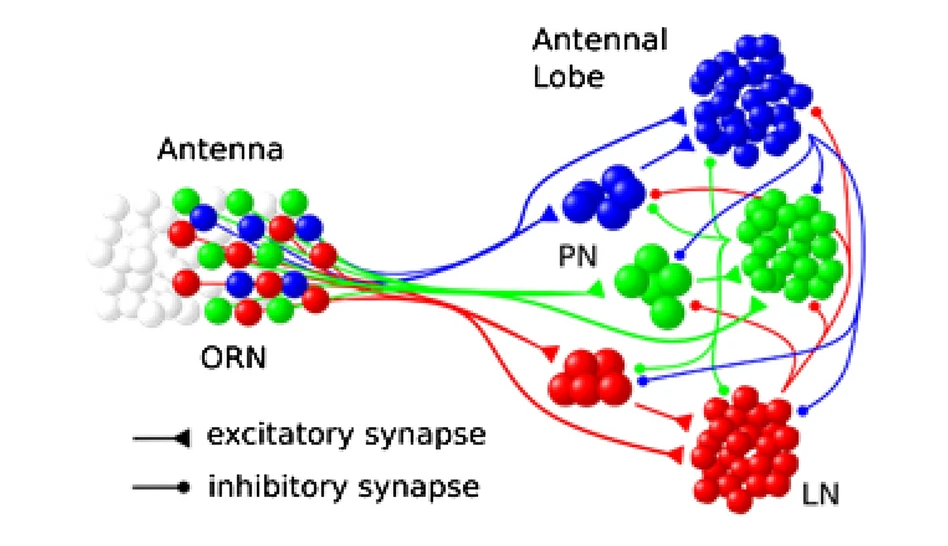
\includegraphics[width=0.8\textwidth]{antennal_lobe_organization}
    \caption{Schematic representation of the antennal lobe of the honey bee, image taken from \cite{bee-geosmin}.}
    \label{fig:antennal-lobe}
  \end{figure}

  \subsection{Antennal lobe}
  The antennal lobe is the first olfactory neuropil of the bee brain and its organization can be seen in figre \ref{fig:antennal-lobe}.
  It is composed of about 160 glomeruli, spherical structures of about 30 micrometers in diameter.
  The glomerulus is the functional unit of the AL, where the ORNs expressing the same olfactory receptor converge.
  An odorant creates a stereotypical map of activity in the AL, activating a subset of glomeruli.
  The neurons of the antennal lobe can be classified into two species: the local interneurons (LNs) and the projection neurons (PNs) \cite{bee-atlas}.
  Within a glomerulus sensory afferents form synapses with local interneurons and projection neurons.
  The olfactory receptor neurons convey odor, mechanosensory and gustatory information to the rest of the antennal lobe.
  They enter the AL through the antennal nerve and terminate in the glomeruli.
  Furthermore, each antenna innervates only the ipsilateral side and innervation is antennotropic: afferents originating in the distal flagellomeres occupy the external margin of the glomerular cortex, while proximal segments the inner one.

    \subsubsection{Local interneurons}
    Local interneurons arborize through the whole glomerular volume and form synapses with the projection neurons \cite{local-neurons}.
    They can present a similar density of arborization among all innervated glomeruli, or a dense arborization in one particular glomerulus.
    Their activity is odor-specific, they receive input from the glomerulus and deliver a mostly inhibitory output to other glomerulus.
    Their inhibitory activity is towards glomeruli in a spatial discontinuous pattern mediated by GABAergic synapses.
    This inhibitory effect of the LN produces a reduction in response intensity and a spatial and temporal increase in the representation power of the projection neurons' activity.

    \subsubsection{Projection neurons}
    Projection neurons are responsible for relaying the processed olfactory information to higher-order processing centers.
    Most of them receive input from individual glomeruli.
    The reduction in population size from the olfactory receptor neurons increases sensitivity and improves signal-to-noise ratio \cite{noise-in-pn}.
    Their dendrites occupy the glomerular inner volume, only partially overlapping with the ORNs' pre-synaptic terminal which occupies the glomerular cortex.
    They innervate the mushroom body and the lateral protocerebrum, in particular the lateral horn.
    Axons leave the LA in five AL tracts ALTs.
    Fibers in these tracts differ in response latency, concentration coding and odorant specificity, suggesting that they may code for different properties of the stimulus \cite{pn-coding}.

\section{Modelling neuronal circuitry}
The study of the brain is a complex task, due to the high number of neurons and their interactions and it requires the use of different techniques and a system-level approach.
The brain is composed of a large number of neurons, each of which is a complex system on its own.
Recent advances in neuroscience have allowed for the study of the brain at a finer scale, but the complexity of the system still poses a challenge.
The work proposed here involves the creation of a spiking recurrent neural network model of the antennal lobe, which will be fine-tuned to replicate the activity of the biological system.\\
This computational model has several advantages over an experimental approach, allowing for a more detailed data collection and study of the system, both in areas where data is available and in the frequency at which data is collected from the system.

  \subsection{Functional representation of a biological neuron}
  A biological neuron is a complex system that can be functionally divided into three parts: the dendrites, the soma and the axon (see figure \ref{fig:neuron-anatomy}).

  \begin{figure}
    \centering
    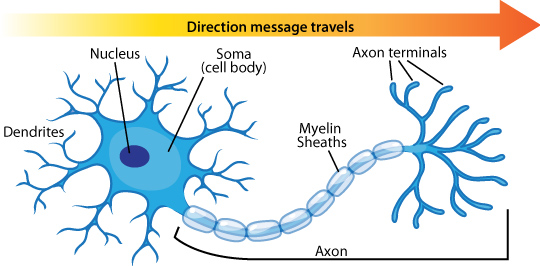
\includegraphics[width=0.8\textwidth]{neuron_anatomy}
    \caption{Schematic representation of the neuron, image taken from \cite{neuron-anatomy-schema}.}
    \label{fig:neuron-anatomy}
  \end{figure}

  The dendrites are the input part of the neurons, that collects signals from others and transmits them to the soma.
  The soma is the ``central processing unit'' of the neuron, where the signal is transformed in a non-linear way: if the total input exceeds a certain threshold an output signal is generated.
  The output signal is then in turn taken over by the axon, which delivers it to other neurons \cite{neuronal-dynamics}.

    \subsubsection{Spike trains}
    The neuronal signal consists of short electrical pulses, which are called action potentials or spikes.
    These spikes have an amplitude of around $100mV$ and a duration in the order of a few milliseconds.
    The form of the pulse is constant when it travels along the axon and it tends to be similar among different neurons.
    Spikes can be fired at regular or irregular intervals in a neuron, depending on the input signal.
    From this information, it can be safely inferred that it is the number and timing of spikes that carry the information representation power in the brain and that a single action potential is the elementary unit of transmission.

    \subsubsection{Synapses}
    Synapses are the places where two neurons come in contact: the axon of a neuron (called pre-synaptic) reaches the dendrites or soma of another (called post-synaptic).
    The most common type of synapse in the brain is the chemical synapse.
    In this type of synapse the axon terminal of the pre-synaptic neuron leaves only a tiny gap with the post-synaptic cell membrane, the synaptic cleft.
    When an action potential arrives at a synapse, it triggers a chain of biochemical processing steps that results in the release of neurotransmitters in the synaptic cleft.
    As soon as the neurotransmitter reaches the post-synaptic membrane it will bind to specific receptors, which will in turn open ion channels causing a change in the membrane potential of the post-synaptic neurons.\\
    Synapses then have a two-fold function: they transmit the signal between neurons and convert it from electrical to chemical and back to electrical, possibly causing another set of non-linear transformations to it.

  \subsection{Modelling neurons - the leaky integrate and fire model}
  One of the most widely used models for analyzing the behavior of neural systems is the leaky integrate-and-fire model.
  The membrane potential of a neuron is described in terms of the synaptic inputs and the injected current that it receives \cite{lif-review}.
  An action potential is generated when the membrane potential reaches a threshold.
  In a sense, a neuron is an integrator of the incoming current and is equated to a capacitor-resistance electric circuit, as seen in figure \ref{fig:lif-circuit}.
  This is a point-neuron model: the spatial structure of the neuron associated with the dendrites is neglected.

  \begin{figure}
    \centering
    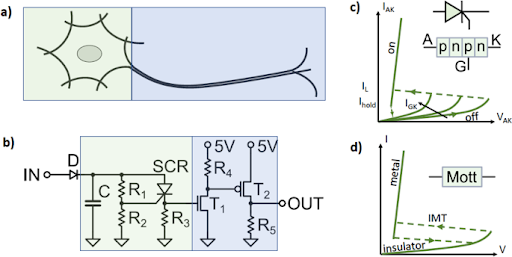
\includegraphics[width=0.8\textwidth]{lif-schema}
    \caption{Modelling a neuron as a integrate and fire model, image taken from \cite{lif-schema}.}
    \label{fig:lif-circuit}
  \end{figure}

  The input can modelled as either injected currents (current synapses model, summation is linear) or as changes in the membrane conductance (conductance synapses model, summation is non-linear),  weighted by the respective synaptic strength.\\
  The model is leaky because the summed contributions to the membrane potential decay with a characteristic time constant.\\
  The neuron generates a spike (or fires) when the membrane potential reaches a fixed threshold value.
  When this happens the membrane potential is reset to a standard resting value and, in some cases, it becomes refractory for a certain period of time.
  The generation of an action potential is generally not considered an intrinsic part of the model: it is usual in the description of this model to model only sub-threshold behavior.\\
  It can be seen how the fundamental variable describing the dynamics of the neuron is the membrane potential, which evolves in time according to:

  \begin{equation}
    C_m\frac{dV(t)}{dt} = I_{leak}(t) + I_{syn}(t) + I_{inj}(t)
    \label{eq:lif-membrane-potential}
  \end{equation}

  Where $C_m$ is the membrane capacitance and is related to the time constant of decay, $I_{leak}(t)$ is the current due to the passive leak of the membrane $I_{syn}(t)$ is a current describing the effect of the synaptic input to the neuron and $I_{inj}(t)$ is a current injected into the neuron.
  The behavior of the simplest iteration of a leaky integrate and fire neuron can be seen in figure \ref{fig:lif-behavior}.

  \begin{figure}
    \centering
    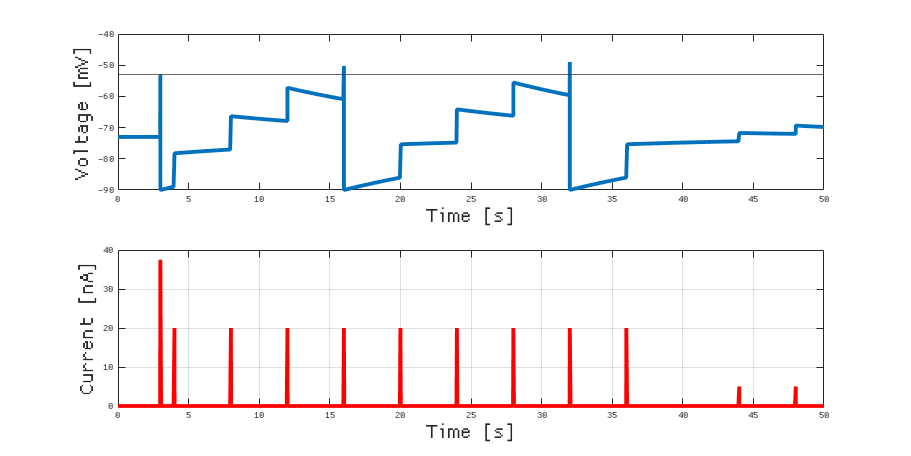
\includegraphics[width=0.8\textwidth]{lif-behavior}
    \caption{Behavior of the simplest leaky integrate and fire neuron: $\begin{cases} \frac{dV(t)}{dt} = -\frac{V(t)}{\tau_m} + I_{inj} \\ V(t) = V_{reset} \text{ if } V(t) \geq V_{th} \end{cases}$, generated with MatLab \cite{matlab}.}
    \label{fig:lif-behavior}
  \end{figure}

  The input currents can be further described as:

  \begin{equation}
    I_{leak}(t) = -\frac{C_m}{\tau_m}\left[V(t) - V_{rest}\right]
  \end{equation}

  Where $V_{rest}$ is the resting potential of the neuron and $\tau_m = R_mC_m$ is the membrane time constant, the product of the membrane capacitance and the leak resistance.\\
  Although not necessary the spiking mechanism can be included in the model in terms of a spiking current:

  \begin{equation}
    I_{spike}(t) = C_m\left[\frac{dV(t)}{dt}\right]^{-1}_{v = V_{th}}\left(V_{reset}-V_{th}\right)\delta\left[V(t)-V_{th}\right]
  \end{equation}

  This equation describes a spike when the membrane potential reaches the spike generating threshold $V_{th}$, which is followed by a reset of the membrane potential to $V_{reset}$.
  $\delta$ denotes the Dirac delta function.
  The membrane potential begins to evolve again according to equation \ref{eq:lif-membrane-potential} after an absolute refractory period, which can be $0$ for certain applications.

    \subsubsection{Current synapses}
    The synaptic current for a current synapse is independent of the membrane potential and is described by:

    \begin{equation}
      I_{inj}(t) = C_m\sum\limits_{k=1}^{N_E}a_{E,k}S_{E,k}(t) + C_m\sum\limits_{k=1}^{N_I}a_{I,k}S_{I,k}(t)
    \end{equation}

    Where $a_{E,k}>0$ and $a_{I,k}<0$ are the change in potential due to a single synaptic event and when multiplied by $C_m$ form the associated charge delivered to the neuron by an excitatory and inhibitory input respectively.
    $S_{E,k}(t)$ and $S_{I,k}(t)$ describe the spike train:

    \begin{equation}
      S_{E,k}(t) = \sum\limits_{t_{E,k}}\delta(t-t_{E,k})\qquad S_{I,k}(t) = \sum\limits_{t_{I,k}}\delta(t-t_{I,k})
    \end{equation}

    Where $t_{E,k}$ and $t_{I,k}$ are the spike times of the $k$-th excitatory and inhibitory synapses respectively.

    \subsubsection{Conductance synapses}
    Conductance synapses offer a more biologically accurate description of synaptic current.
    They are modeled as:

    \begin{align}
      I_{syn}(t) &= C_m\left[V_E-V(t)\right]\sum\limits_{k=1}^{N_E}g_{E,k}S_{E,k}(t) + C_m\left[V_I-V(t)\right]\sum\limits_{k=1}^{N_I}g_{I,k}S_{I,k}(t)
    \end{align}

    Where $V_E$ and $V_I$ are the reversal potentials, which arise from the equilibrium potentials of the ion channels.
    The direction of the associated current flow switches when the membrane potential crosses the reversal potential.
    They introduce a non-linear factor into the summation of the individual synaptic inputs.
    $g_{E,k}\land g_{I,k}>0$ are the integrated conductances over the time course of the synaptic events divided by the neural capacitance (so they are dimensionless).

  \subsection{Interacting neurons - spiking neural networks}
  A collection of leaky integrate and fire neurons can be aggregated into a network.
  In this way, a spiking neural network (SNN) is formed.
  Spiking neural networks offer a different perspective on machine learning with respect to classical artificial neural networks (ANN) \cite{snn-review}.
  Data is encoded in a series of discrete time spikes, which mimics a biological brain more closely than ANNs, introducing several layers of complexity.
  First of all, information is no longer coded as a continuous function but as a series of discrete events (the spike train): it is the frequency of spikes and their precise timing that becomes the information carried along the network.
  The leaky integrate and fire (LIF) neurons become the fundamental unit of the network.
  Both classical artificial units and LIF units perform a non-linear transformation of the input, but the LIF unit holds a state (the membrane potential), introducing a sort of memory at a unit's level.
  Memory is also introduced at a system level: a biological brain is rich in recurrent connections, disrupting the classical layer structure of classical ANNs.
  A summary of the differences between classical ANNs and SNNs can be seen in figure \ref{fig:ann-vs-snn}.

  \begin{figure}
    \centering
    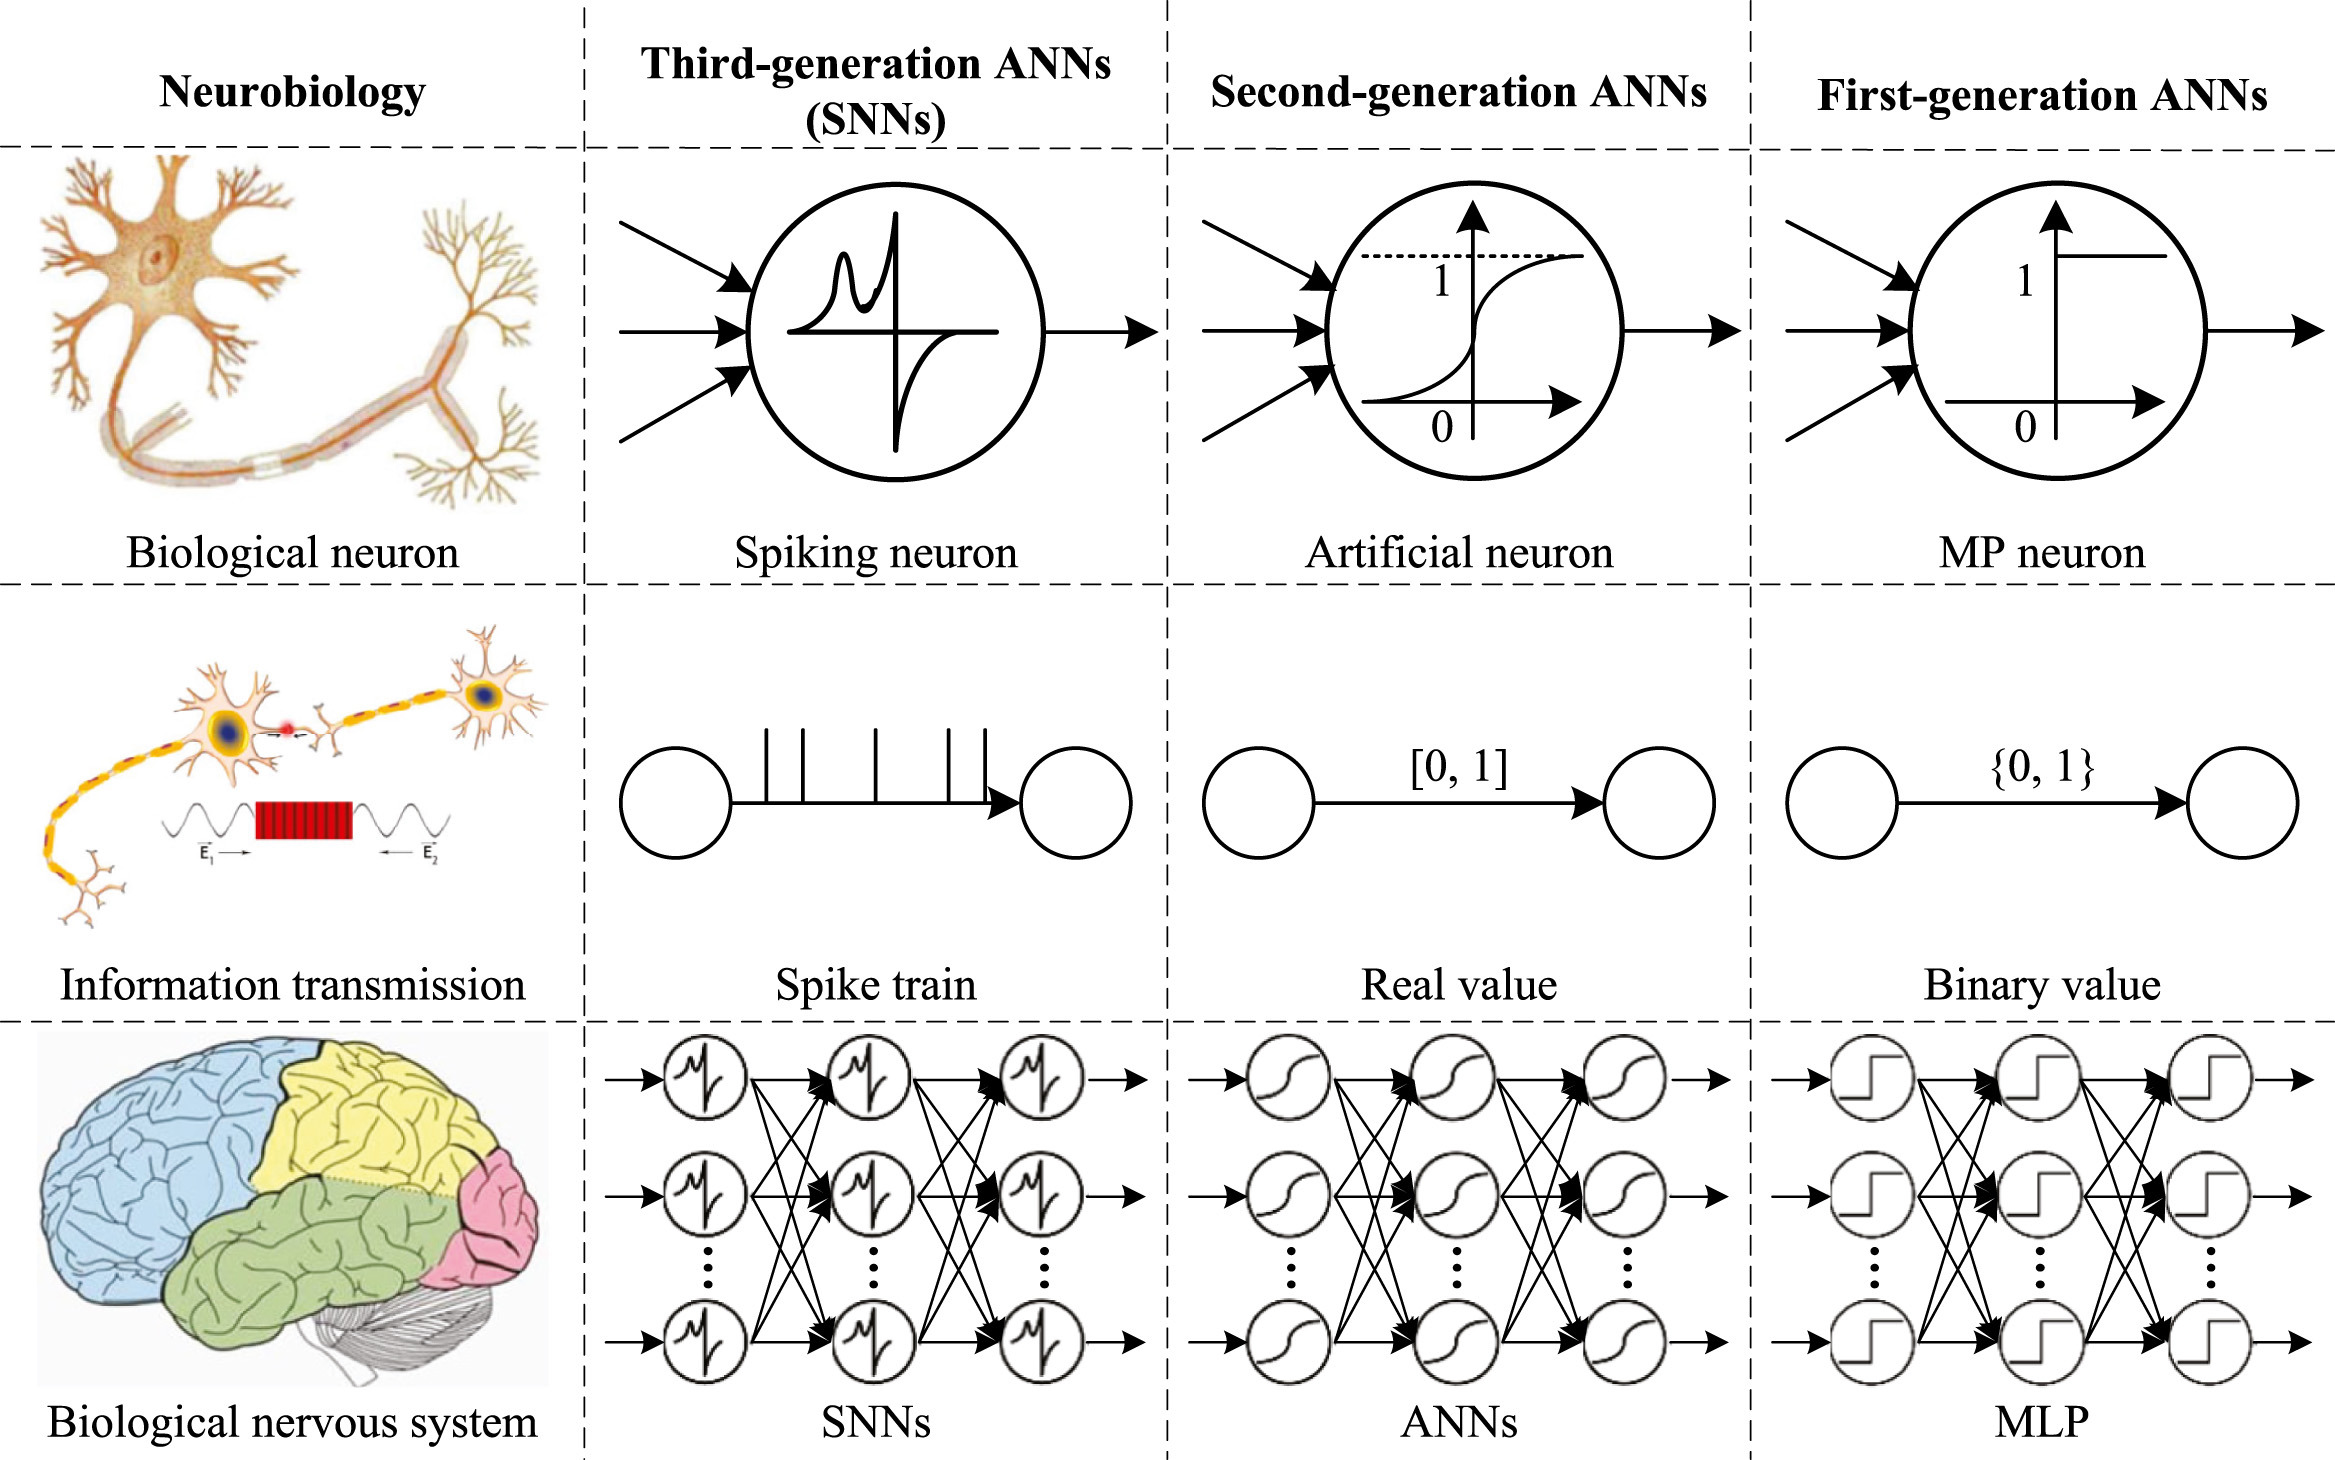
\includegraphics[width=0.8\textwidth]{ann-vs-snn}
    \caption{Schematic representation of the major differences between ANNs and SNNs. Image taken from \cite{ann-vs-snn}.}
    \label{fig:ann-vs-snn}
  \end{figure}

  This is interesting because biological brains are striking in how much more predictive power and efficiency they have with respect to ANNs: despite the potentially massive parameter space, the human brain only consumes about $20W$.\\
  It's this massive superiority that makes biological networks so riveting to study and model and why spiking neural networks are becoming more and more popular in machine learning.
  This impressive space and energy efficiency is due to the fact that most neurons are usually inactive, meaning that the brain is highly sparse.
  SNNs attempt to combine more biologically plausible inputs, learning methods and architectures in order to match ANNs' performance while achieving the energy efficiency and robustness of the human brain.\\
  From an optimization point of view, SNNs pose a unique challenge as they lack interpretable models, straightforward gradient calculation and methods that leverage the inherent advantages of SNNs.
  It's because of this lack of methods that observing biological networks is so important: it can provide insight into the inner workings of the brain and can be used to develop new methods for SNNs.\\
  The work presented here is an attempt to open the ``black box'' of SNNs and try to understand their dynamics and how they can be used to solve problems.
  To do so a combination of mathematical analysis and numerical simulation will be used together with system neuroscience methods to investigate the dynamics of a specific SNN.
  The availability of experimental data will allow to fine-tune the model and to compare the results of a simulation with them, offering a way to validate the model, while still allowing to change it to try to understand the effect of the single elements of the system on its behavior.

\section{Code availability}
All the code used to generate the results presented in this work is available at \href{https://github.com/giacThePhantom/genn-network-model}{https://github.com/giacThePhantom/genn-network-model}.
